\chapter{Implementation and Development}
\label{chap:implementation}

\section{Module 1: GitHub App Authentication and Token Management Service}
\label{sec:impl-github-auth}

\noindent\textbf{Source Files:} \texttt{backend/app/services/github/auth.py} and \texttt{client.py}

The GitHub authentication subsystem manages asymmetric cryptographic keys, JSON Web Token (JWT) minting, and installation access token resolution. Figure~\ref{fig:github-auth-workflow} depicts the complete token minting workflow.

\begin{figure}[htbp]
    \centering
    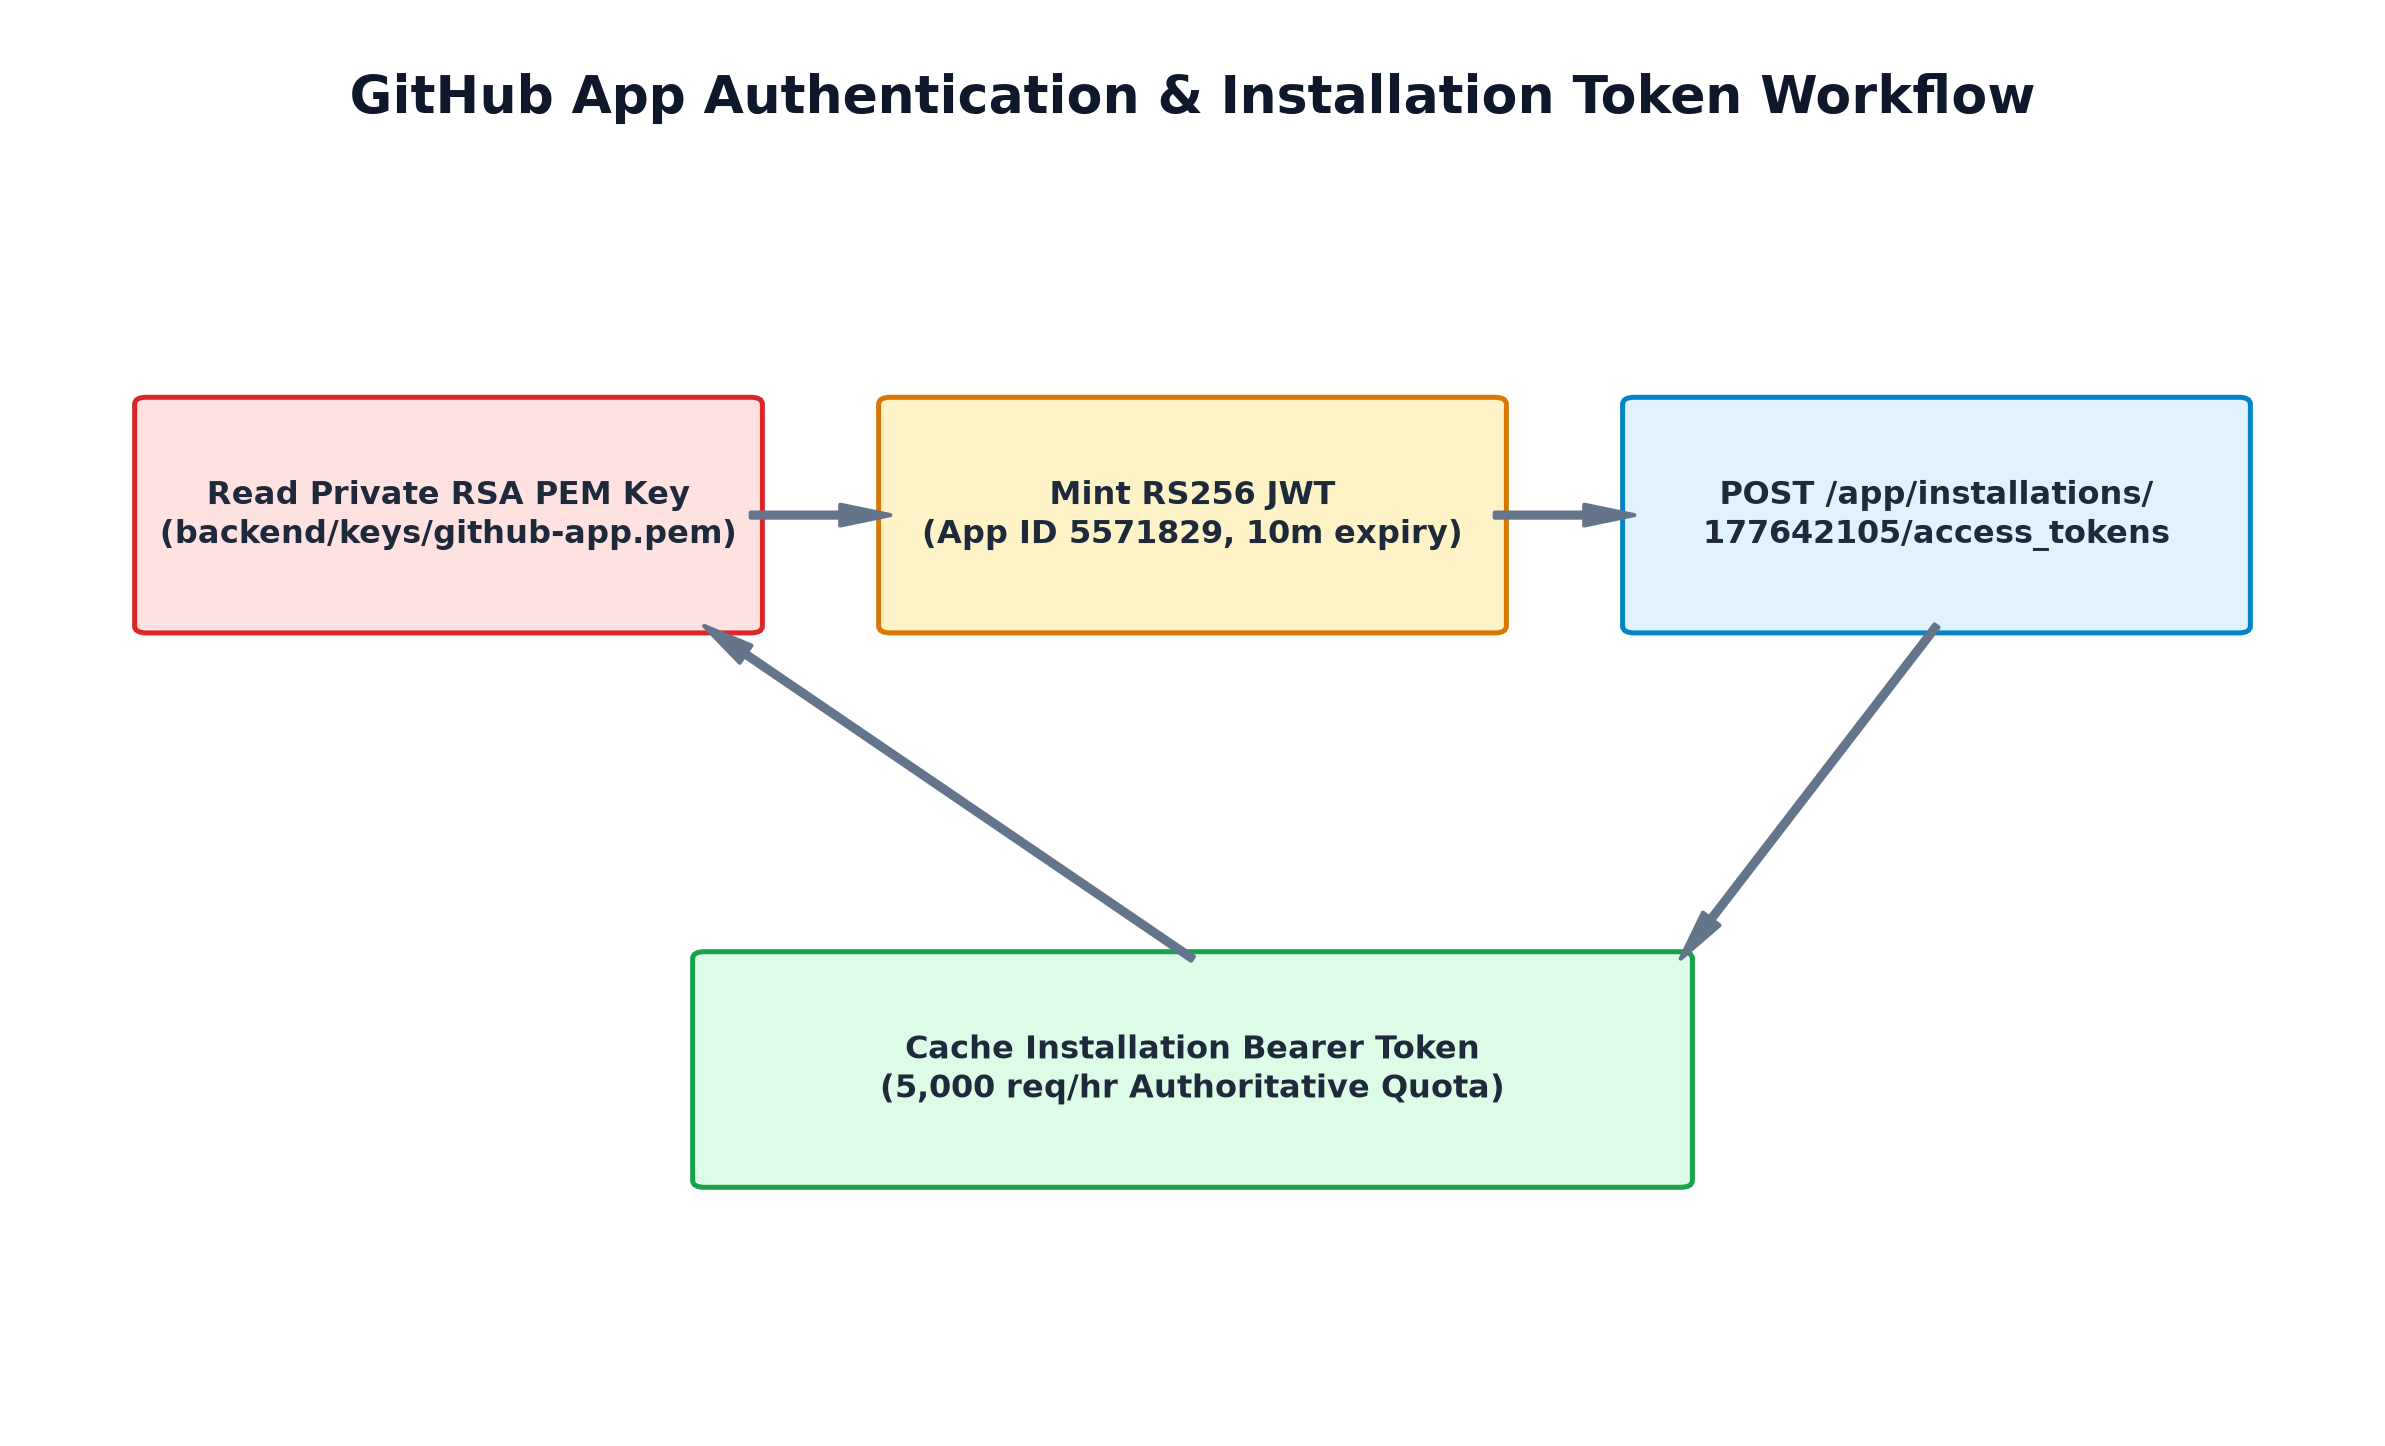
\includegraphics[width=0.88\textwidth]{images/workflows/github_auth_workflow.png}
    \caption{GitHub App Authentication and Installation Token Workflow}
    \label{fig:github-auth-workflow}
\end{figure}

The service initializes by loading the GitHub App private RSA key from \texttt{backend/keys/github-app.pem}. When invoked, \texttt{create\_jwt()} generates an RS256-signed JWT with a 10-minute validity window containing App ID \texttt{5571829}:

\begin{lstlisting}[language=Python, caption={RS256 JWT Generation in GitHub Auth Service}]
def create_jwt() -> str:
    now = int(time.time())
    payload = {
        "iat": now - 60,
        "exp": now + (10 * 60),
        "iss": settings.GITHUB_APP_ID
    }
    with open(settings.GITHUB_APP_PRIVATE_KEY_PATH, "r") as f:
        private_key = f.read()
    return jwt.encode(payload, private_key, algorithm="RS256")
\end{lstlisting}

Crucially, to prevent rate limit exhaustion when endpoints query repository data without user-supplied tokens, MergeMind implements \texttt{get\_default\_token()}. This function automatically resolves installation ID \texttt{177642105} and injects the installation bearer token into \texttt{GitHubClient} session headers. Consequently, all repository queries operate against GitHub's authoritative 5,000 requests/hour enterprise pool (verified with 4,986 remaining quota).

\section{Module 2: Webhook Signature Verification and Event Dispatcher}
\label{sec:impl-webhooks}

\noindent\textbf{Source File:} \texttt{backend/app/api/v1/endpoints/webhooks.py}

The webhook dispatcher receives asynchronous HTTP POST callbacks from GitHub at \texttt{/api/v1/webhooks/github}. To guarantee cryptographic non-repudiation and prevent spoofing attacks, incoming requests are validated against the \texttt{X-Hub-Signature-256} header. The raw request body bytes are hashed using HMAC-SHA256 parameterized with \texttt{settings.GITHUB\_WEBHOOK\_SECRET}:

\begin{lstlisting}[language=Python, caption={Cryptographic HMAC-SHA256 Webhook Verification}]
expected_signature = "sha256=" + hmac.new(
    settings.GITHUB_WEBHOOK_SECRET.encode("utf-8"),
    raw_body,
    hashlib.sha256
).hexdigest()

if not hmac.compare_digest(expected_signature, request_signature):
    raise HTTPException(status_code=401, detail="Invalid webhook signature")
\end{lstlisting}

Verified payloads are routed based on the \texttt{X-GitHub-Event} header: \texttt{push} events trigger cache invalidation; \texttt{pull\_request} events trigger automated AI PR review pipelines; and \texttt{workflow\_run} events (with \texttt{conclusion: 'failure'}) automatically initiate CI failure ingestion and remediation loops, as illustrated in the sequence diagram in Figure~\ref{fig:seq-webhook}.

\begin{figure}[htbp]
    \centering
    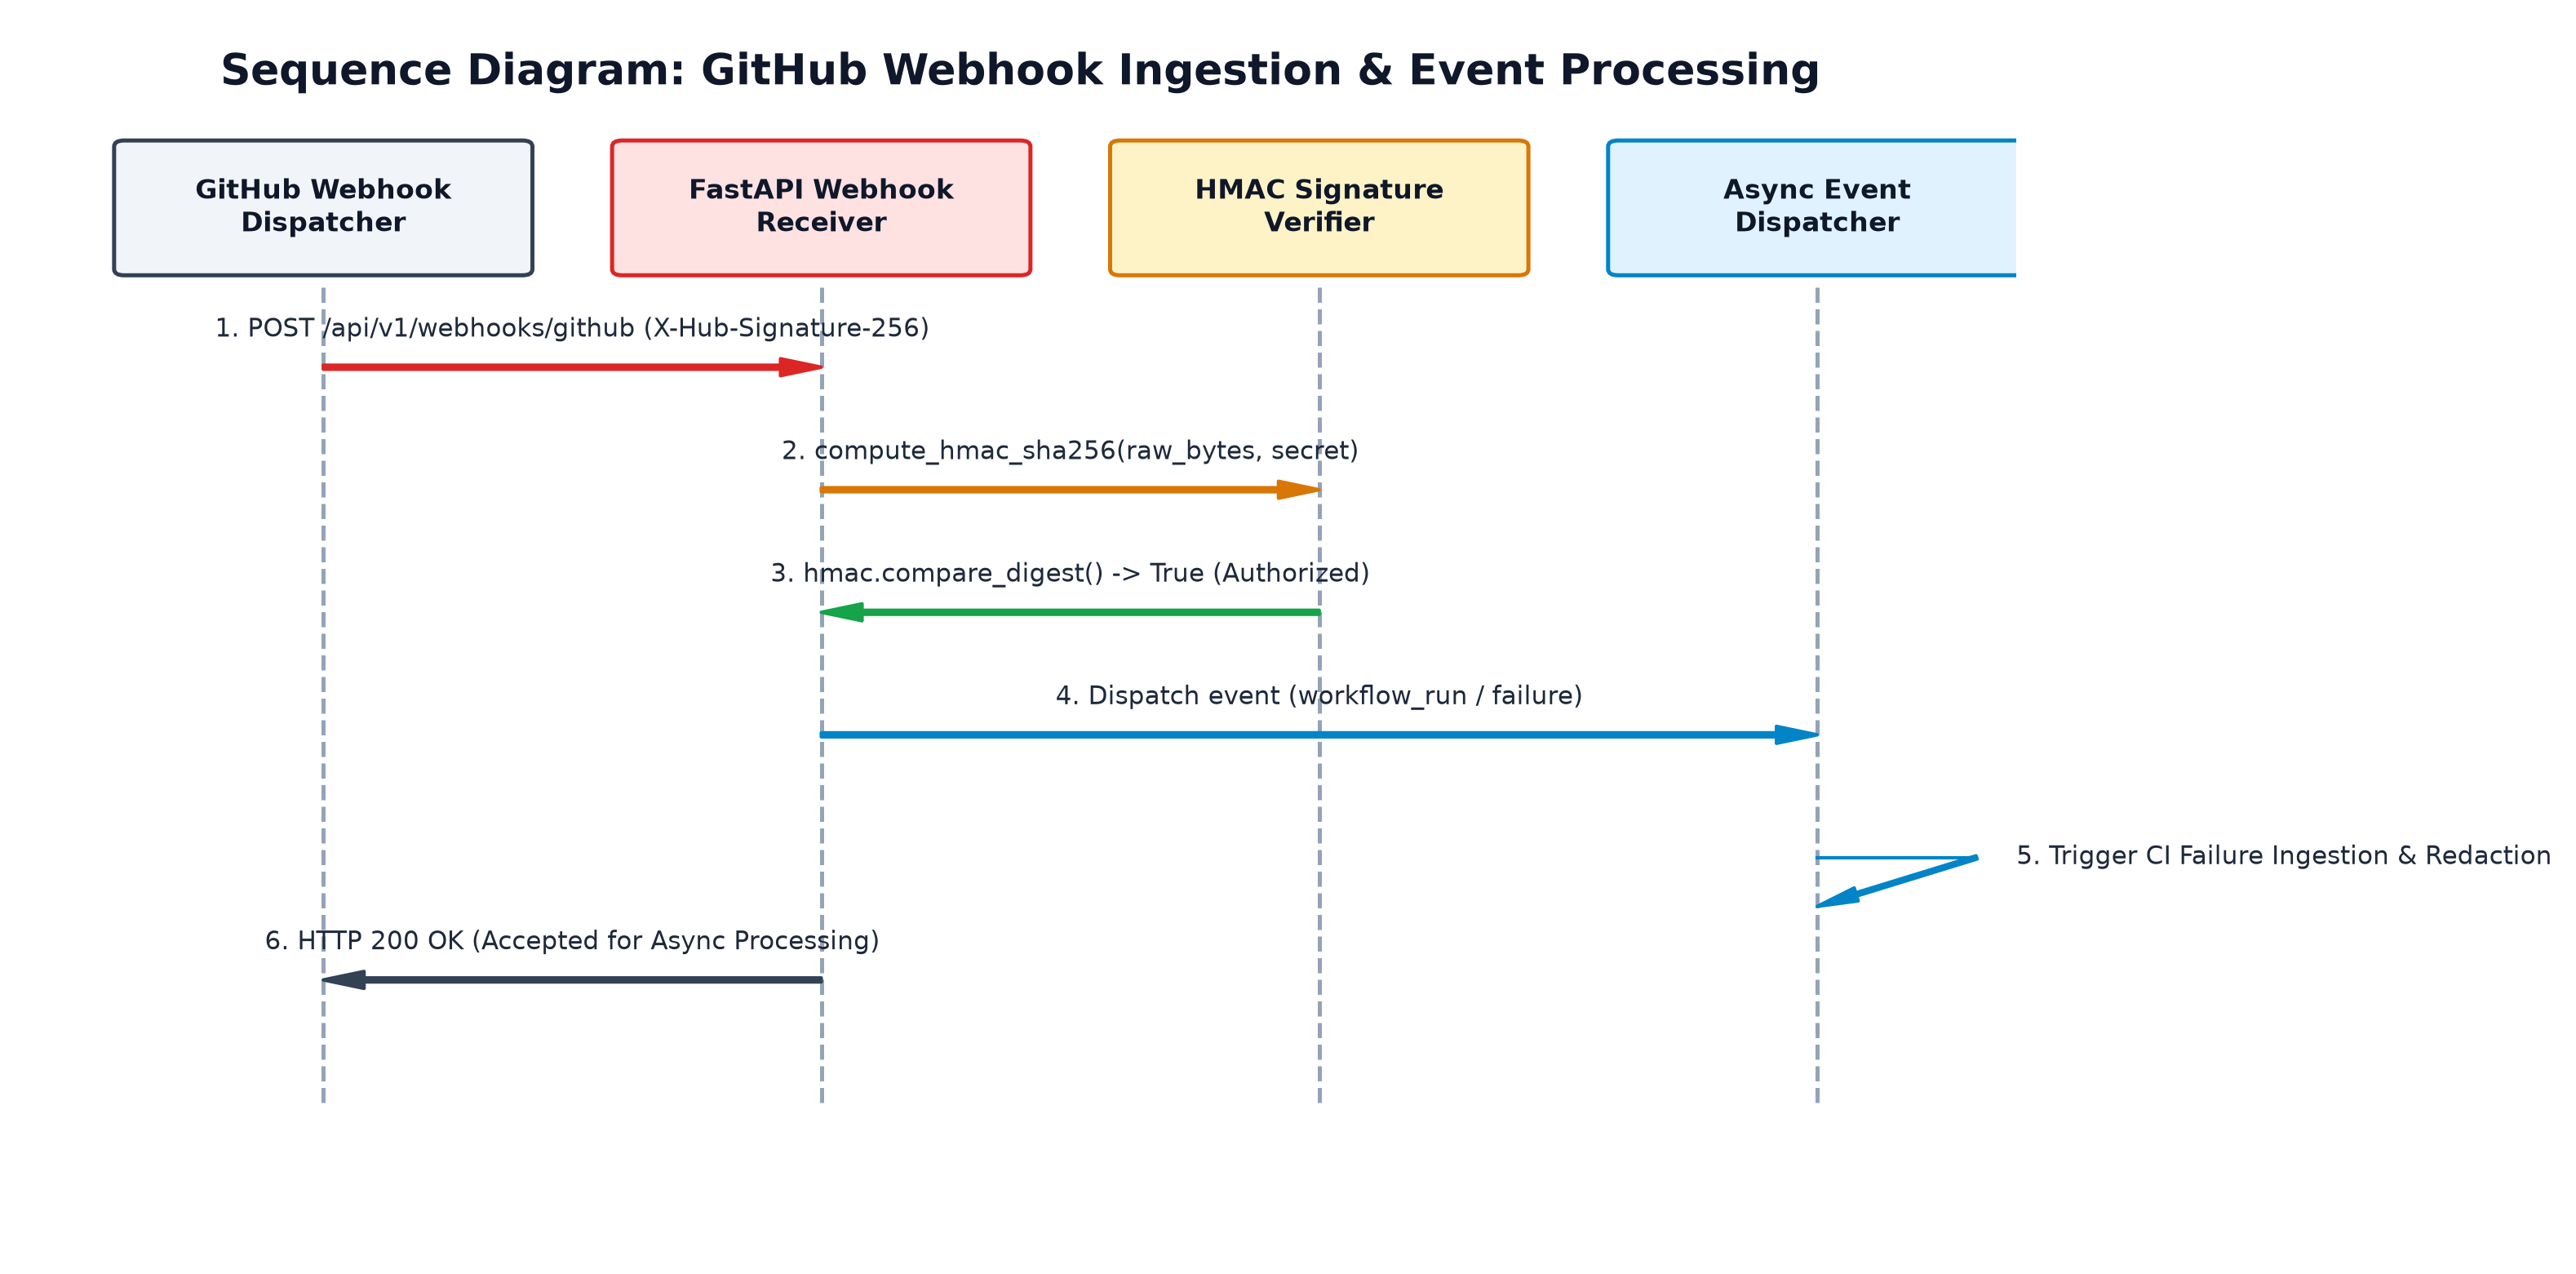
\includegraphics[width=0.90\textwidth]{images/diagrams/sequence_diagram_webhook.png}
    \caption{Sequence Diagram: GitHub Webhook Ingestion and Event Processing}
    \label{fig:seq-webhook}
\end{figure}

\section{Module 3: Dynamic Tarball Ingestion and Sandbox Extractor}
\label{sec:impl-tarball}

\noindent\textbf{Source File:} \texttt{backend/app/api/v1/endpoints/health_assessment.py}

To eliminate cross-repository directory contamination (where previous versions mistakenly scanned the backend container's own working directory \texttt{os.getcwd()}), MergeMind dynamically streams the target repository's source archive directly from GitHub's REST endpoint \texttt{GET /repos/\{owner\}/\{repo\}/tarball/\{branch\}}. 

The streaming response is decompressed in-memory via Python's \texttt{tarfile} module into an ephemeral temporary directory created via \texttt{tempfile.mkdtemp(prefix='mergemind\_repo\_')}. Security validation ensures that no extracted tar member escapes the temporary directory boundary (mitigating Zip Slip path traversal attacks):

\begin{lstlisting}[language=Python, caption={Safe Streamed Tarball Extraction with Path Traversal Defense}]
response = await client.get(f"/repos/{owner}/{repo}/tarball/{branch}")
with tempfile.TemporaryDirectory(prefix="mergemind_repo_") as temp_dir:
    with tarfile.open(fileobj=io.BytesIO(response.content), mode="r:gz") as tar:
        for member in tar.getmembers():
            target_path = os.path.abspath(os.path.join(temp_dir, member.name))
            if not target_path.startswith(os.path.abspath(temp_dir)):
                raise SecurityException("Directory traversal attempt detected in tar archive")
        tar.extractall(path=temp_dir)
    # Execute deterministic linters directly on unpacked temp_dir
    assessment = await runner.run_all_assessments(source_dir=temp_dir)
\end{lstlisting}

Once static analysis completes, the temporary directory is automatically purged from disk, guaranteeing zero cross-repository data contamination.

\section{Module 4: Deterministic Static Code Analysis Harness}
\label{sec:impl-static-harness}

\noindent\textbf{Source File:} \texttt{backend/app/services/health\_assessment/runner.py}

This module coordinates parallel execution of deterministic static analysis tools across the extracted repository snapshot:
\begin{itemize}
    \item \textbf{Astral Ruff Harness:} Executes \texttt{ruff check --output-format=json \{source\_dir\}}, parsing JSON diagnostics to calculate linting violations (Weight: 25\%).
    \item \textbf{Bandit AST Harness:} Executes \texttt{bandit -r \{source\_dir\} -f json}, classifying findings into Severity and Confidence categories (Weight: 25\%).
    \item \textbf{pip-audit SCA Harness:} Scans dependency manifests (\texttt{requirements.txt}, \texttt{Pipfile.lock}) against the OSV vulnerability database (Weight: 20\%).
    \item \textbf{Radon Maintainability Harness:} Statically computes McCabe cyclomatic complexity and Maintainability Index distributions (Weight: 10\%).
    \item \textbf{Dynamic Normalizer:} Rescales total health scores over active dimensions and enforces the 80\% qualification gating threshold.
\end{itemize}

\section{Module 5: Enterprise Security Posture Evaluator}
\label{sec:impl-posture-eval}

\noindent\textbf{Source File:} \texttt{backend/app/services/security\_posture/evaluator.py}

The Security Posture Evaluator implements the 43-check governance framework across Branch Protection, Security Features, Access Control, and Repository Settings. The evaluator queries GitHub's REST API using the authenticated installation token across multiple endpoints:
\begin{itemize}
    \item \texttt{GET /repos/\{owner\}/\{repo\}/branches/\{branch\}/protection} (12 checks)
    \item \texttt{GET /repos/\{owner\}/\{repo\}/community/profile}, \texttt{/dependabot/alerts}, \texttt{/code-scanning/alerts}, \texttt{/secret-scanning/alerts} (9 checks)
    \item \texttt{GET /repos/\{owner\}/\{repo\}/collaborators}, \texttt{/keys}, \texttt{/hooks} (8 checks)
    \item \texttt{GET /repos/\{owner\}/\{repo\}}, \texttt{/actions/permissions}, \texttt{/actions/permissions/workflow} (14 checks)
\end{itemize}

The evaluator constructs a structured dictionary containing check statuses (\texttt{PASS}, \texttt{FAIL}, \texttt{WARN}), severity tags, evidence descriptions, and remediation guidance, while computing the composite Security Posture Index (SPI).

\section{Module 6: CI Failure Ingestion, Payload Reconciliation and Token Redactor}
\label{sec:impl-ci-failure}

\noindent\textbf{Source Files:} \texttt{backend/app/schemas/ci\_failure.py} and \texttt{backend/app/api/v1/endpoints/ci\_failures.py}

When CI/CD pipelines fail, execution logs are ingested either via automated webhooks or manual developer upload. To resolve payload schema discrepancies between legacy frontend versions (which sent \texttt{raw\_logs}) and backend schemas (expecting \texttt{raw\_log}), MergeMind implements a robust Pydantic \texttt{@model\_validator(mode='before')} in \texttt{CIFailureIngestRequest}:

\begin{lstlisting}[language=Python, caption={Pydantic Dual-Schema Payload Reconciliation Validator}]
class CIFailureIngestRequest(BaseModel):
    repository_id: int
    workflow_name: str
    commit_sha: str
    raw_log: str

    @model_validator(mode='before')
    @classmethod
    def reconcile_log_fields(cls, data: Any) -> Any:
        if isinstance(data, dict):
            if "raw_logs" in data and "raw_log" not in data:
                data["raw_log"] = data.pop("raw_logs")
        return data
\end{lstlisting}

Before persistence or LLM transmission, the raw log passes through a regex token sanitizer that strips sensitive credentials:
\begin{itemize}
    \item \textbf{GitHub Tokens:} \texttt{gh[pousr]\_[A-Za-z0-9\_]\{36,255\}} $\to$ \texttt{[REDACTED\_GITHUB\_TOKEN]}
    \item \textbf{AWS Secret Keys:} \texttt{(?i)aws\_secret\_access\_key\textbackslash s*=\textbackslash s*[A-Za-z0-9/+=]\{40\}} $\to$ \texttt{[REDACTED\_AWS\_KEY]}
    \item \textbf{Bearer Tokens:} \texttt{Bearer\textbackslash s+[A-Za-z0-9\textbackslash-\_\textbackslash.]\{20,\}} $\to$ \texttt{Bearer [REDACTED\_TOKEN]}
\end{itemize}

Figure~\ref{fig:ci-ingestion-modal} displays the ingestion interface with active regex sanitization.

\begin{figure}[htbp]
    \centering
    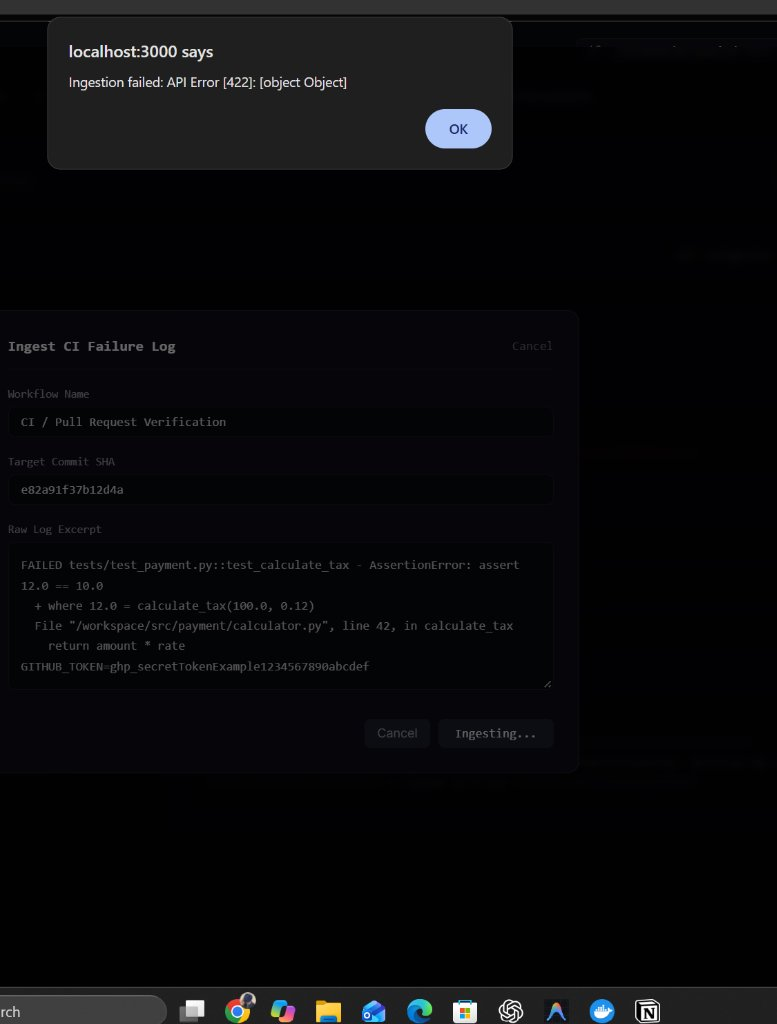
\includegraphics[width=0.75\textwidth]{images/screenshots/ci_failure_ingestion_modal.png}
    \caption{CI Failure Ingestion Modal with Real-Time Regex Secret Redaction}
    \label{fig:ci-ingestion-modal}
\end{figure}

\section{Module 7: AI Remediation Engine and Prompt Synthesis}
\label{sec:impl-remediation}

\noindent\textbf{Source File:} \texttt{backend/app/services/remediation/engine.py}

The remediation engine leverages Google Gemini 3.6 Flash (\texttt{REMEDIATION\_MODEL=gemini-3.6-flash}). The engine parses the sanitized CI failure log to identify the failing assertion or exception trace, extracts the target source file and enclosing function, and constructs a structured system prompt requiring valid Unified Diff format. 

Upon receiving the LLM completion, the engine validates the diff using Python's \texttt{patch} parser and compiles the patched code using Python's \texttt{ast.parse()} to guarantee syntactic validity before sandbox execution. Figure~\ref{fig:pr-review-pipeline} illustrates the AI diff intelligence pipeline.

\begin{figure}[htbp]
    \centering
    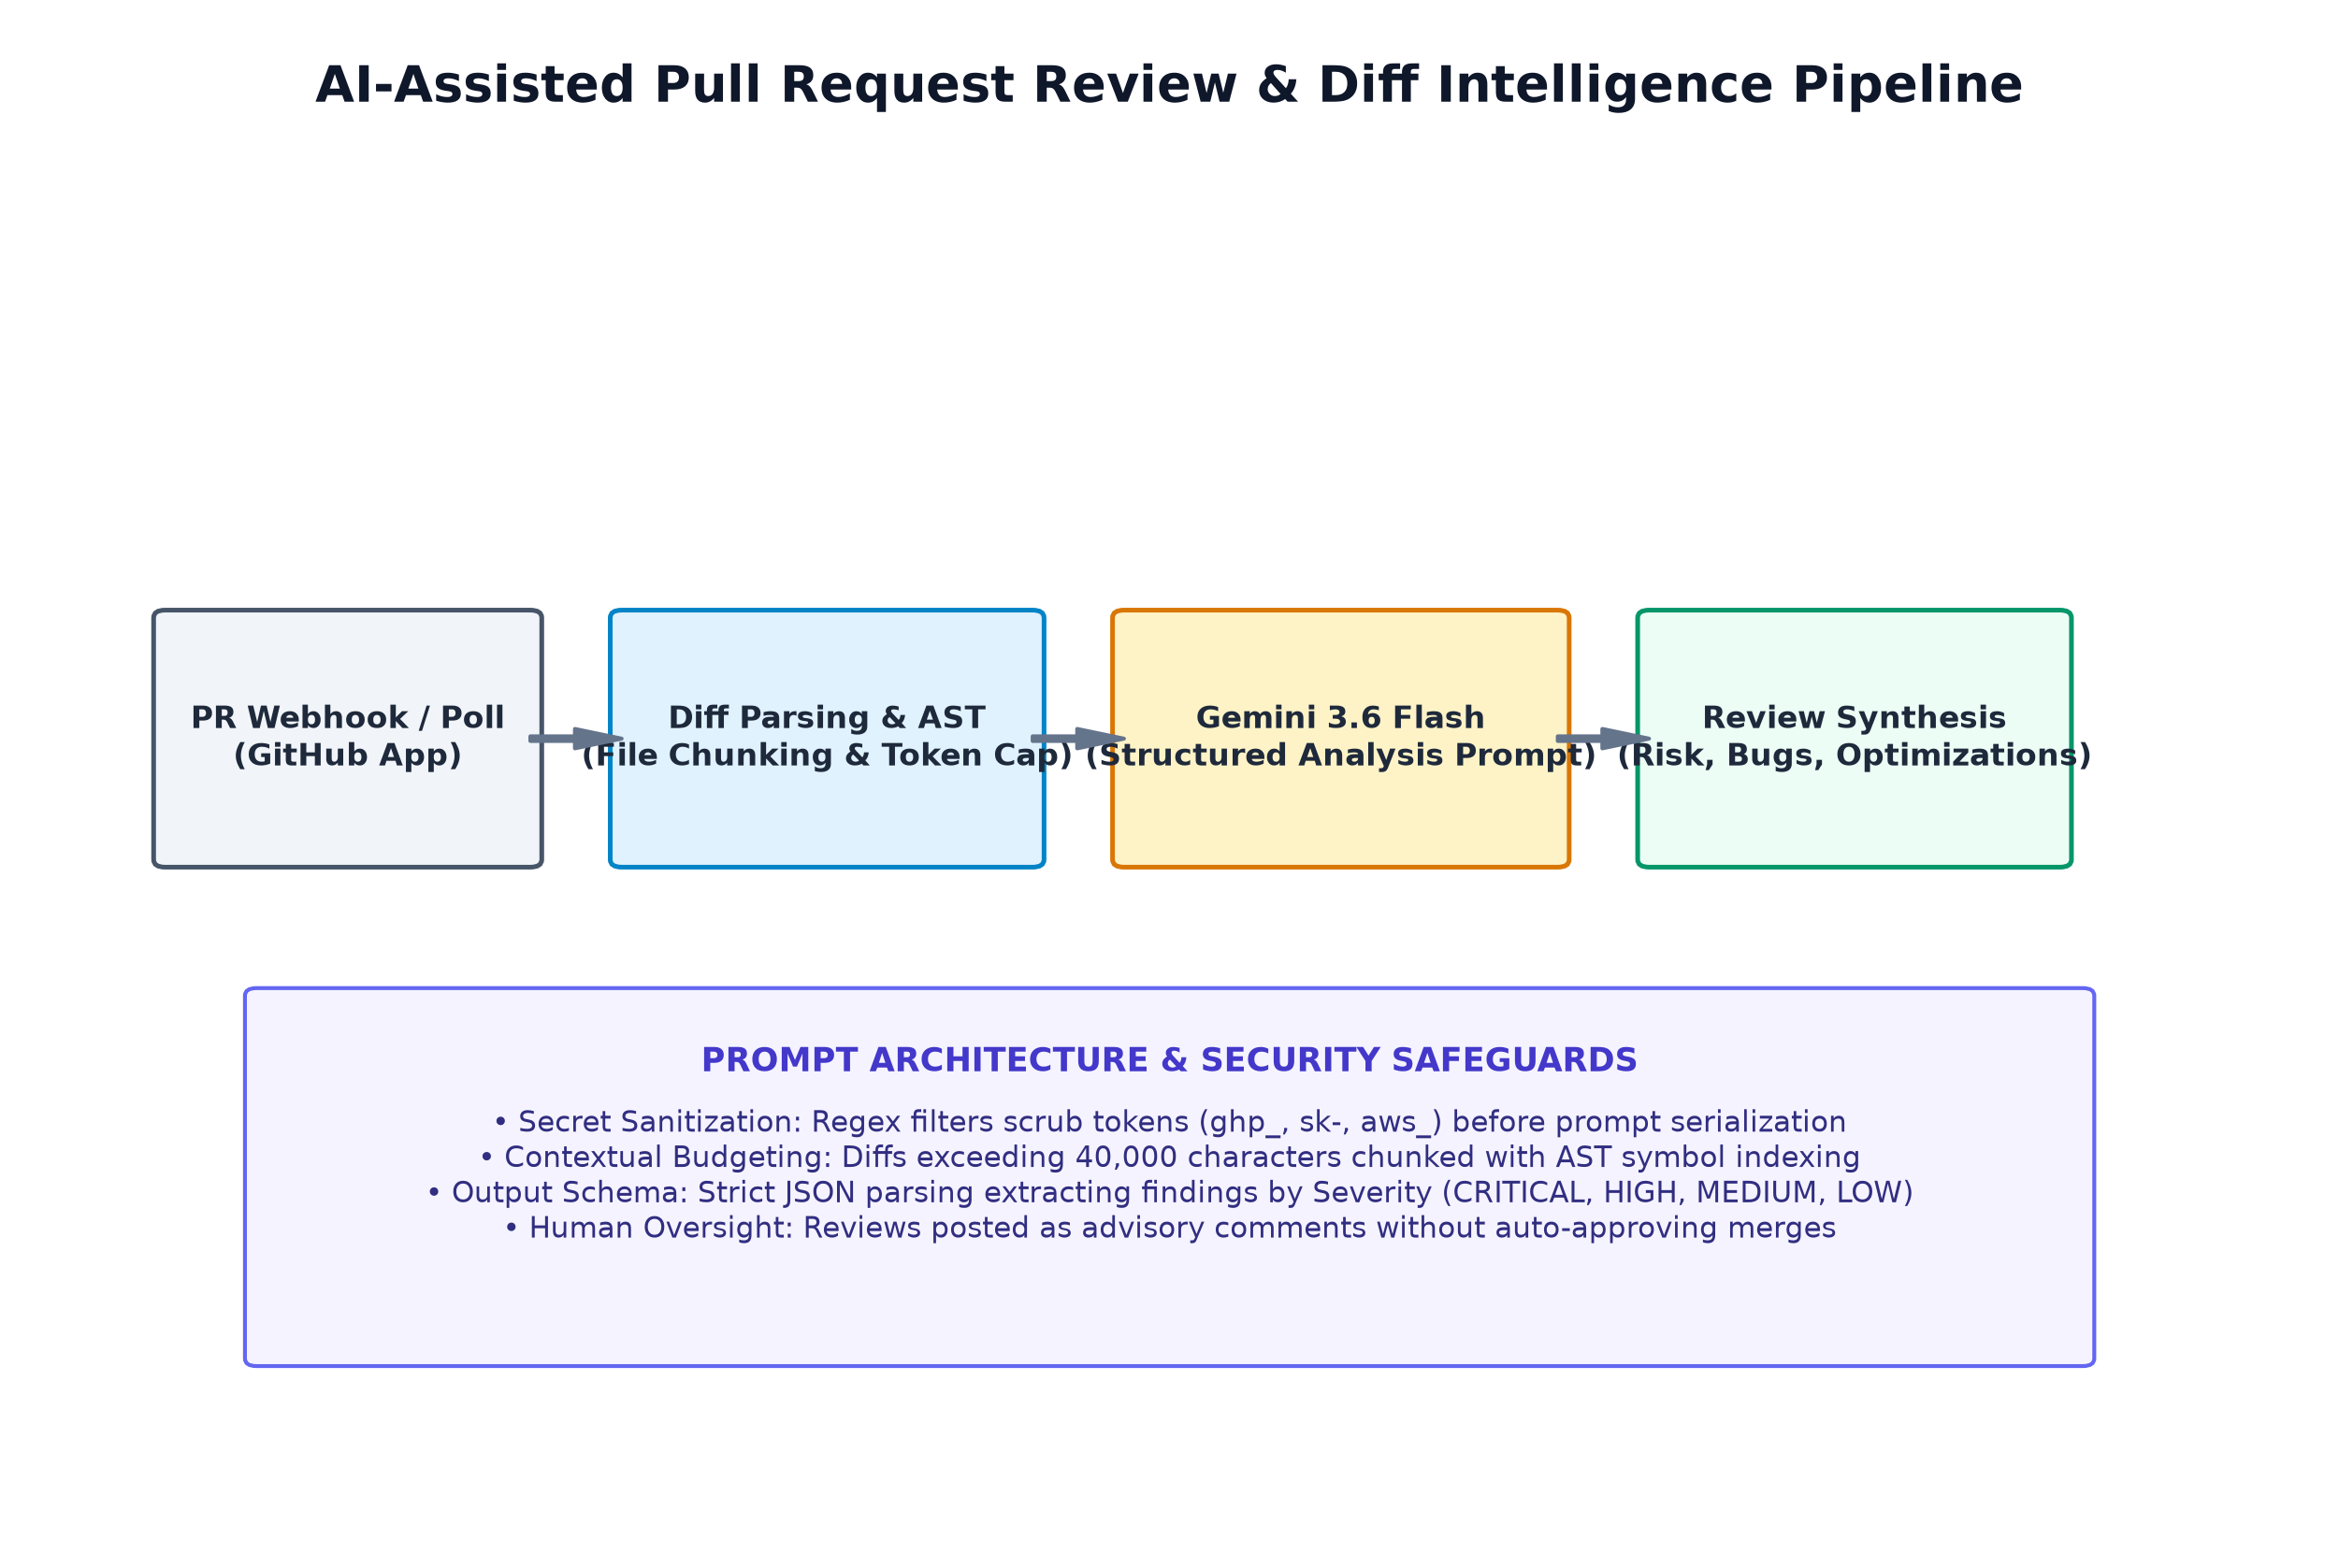
\includegraphics[width=0.90\textwidth]{images/workflows/pr_review_workflow.png}
    \caption{AI Pull Request Review and Contextual Diff Intelligence Pipeline}
    \label{fig:pr-review-pipeline}
\end{figure}

\section{Module 8: Isolated Docker Sandbox Re-Verification and Draft PR Creator}
\label{sec:impl-sandbox-pr}

\noindent\textbf{Source Files:} \texttt{backend/app/services/sandbox/runner.py} and \texttt{pr\_creator.py}

To eliminate hallucinations and prevent untested code merges, candidate patches must pass sandbox re-verification:
\begin{enumerate}
    \item \textbf{Sandbox Execution:} MergeMind spawns an ephemeral Docker container based on \texttt{python:3.11-slim} with dropped Linux capabilities (\texttt{--cap-drop=ALL}), non-root user execution, memory limits (512MB), and read-only container root.
    \item \textbf{Patch Application and Pytest:} The candidate unified diff is applied via \texttt{git apply} or \texttt{patch -p1}. Pytest executes the test suite inside the container.
    \item \textbf{Automated Draft PR Authoring:} If and only if the sandbox test suite exits with code 0 (all tests pass), MergeMind authenticates via the GitHub App installation token, pushes a new remote branch (\texttt{mergemind/fix-ci-\{failure\_id\}}), and opens an official GitHub Draft Pull Request (e.g., Pull Request \#101) containing the diff and AI remediation explanation.
\end{enumerate}

Figure~\ref{fig:remediation-diff-viewer} displays the AI remediation diff viewer confirming verification pass and Draft PR creation.

\begin{figure}[htbp]
    \centering
    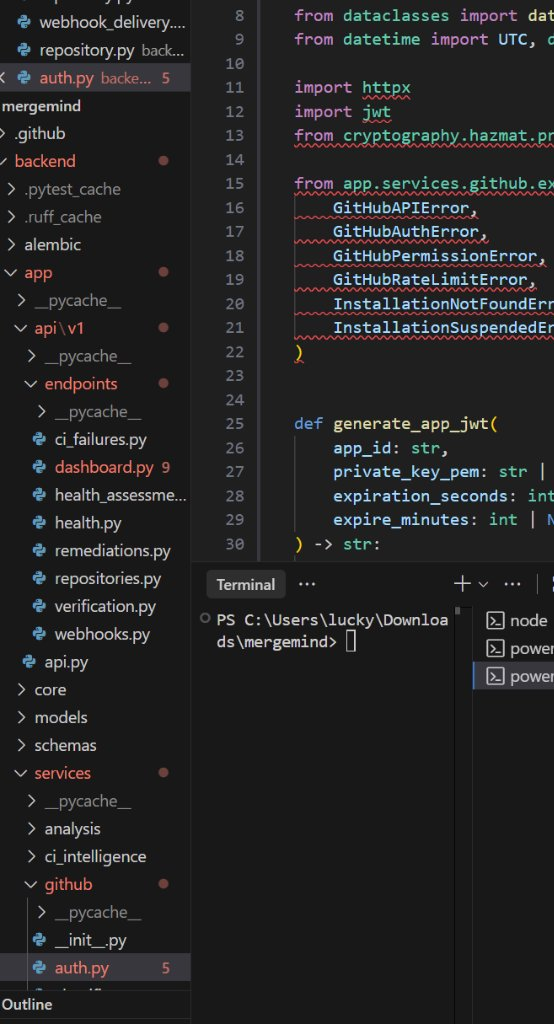
\includegraphics[width=0.75\textwidth]{images/screenshots/remediation_diff_viewer.png}
    \caption{MergeMind AI Remediation Diff Viewer and Verification Output}
    \label{fig:remediation-diff-viewer}
\end{figure}

\section{Frontend Client Architecture and Dashboard Views}
\label{sec:impl-frontend}

The frontend client is implemented in React 18 and TypeScript. The unified API service in \texttt{frontend/src/services/api.ts} automatically injects the \texttt{X-API-Key} header on all outgoing requests. Figure~\ref{fig:ui-dashboard} and Figure~\ref{fig:ui-telemetry-qualified} show the repository overview dashboard and the live multi-factor health telemetry view.

\begin{figure}[htbp]
    \centering
    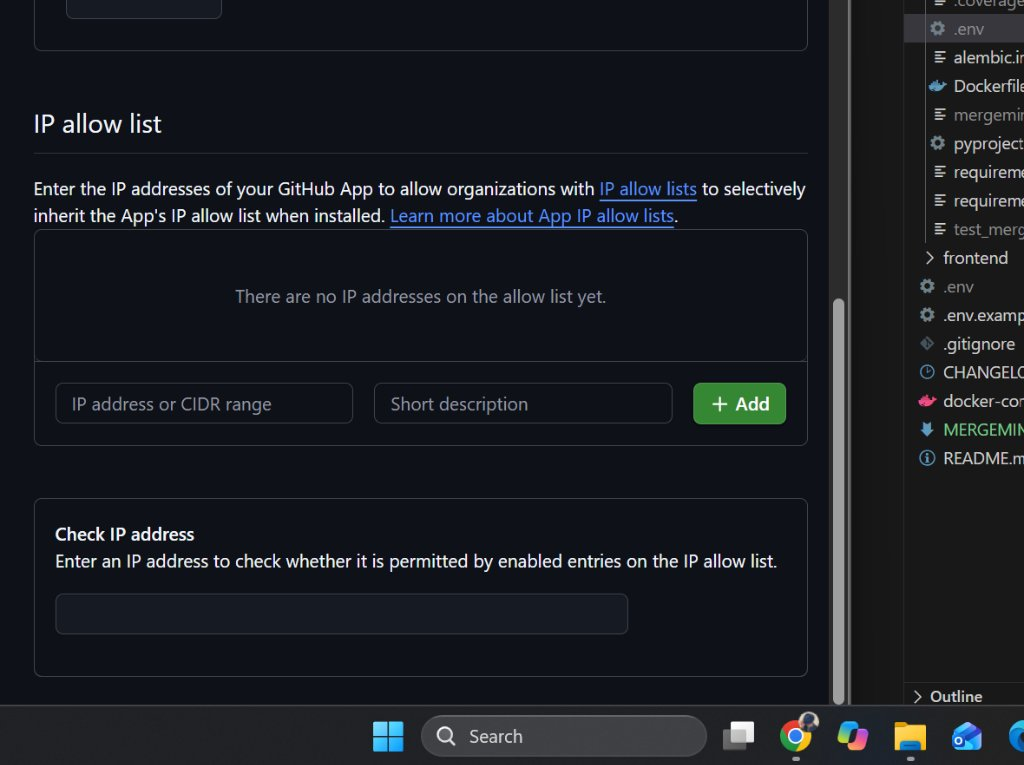
\includegraphics[width=0.88\textwidth]{images/screenshots/dashboard_overview.png}
    \caption{MergeMind Frontend Repository Overview and Health Dashboard Interface}
    \label{fig:ui-dashboard}
\end{figure}

\begin{figure}[htbp]
    \centering
    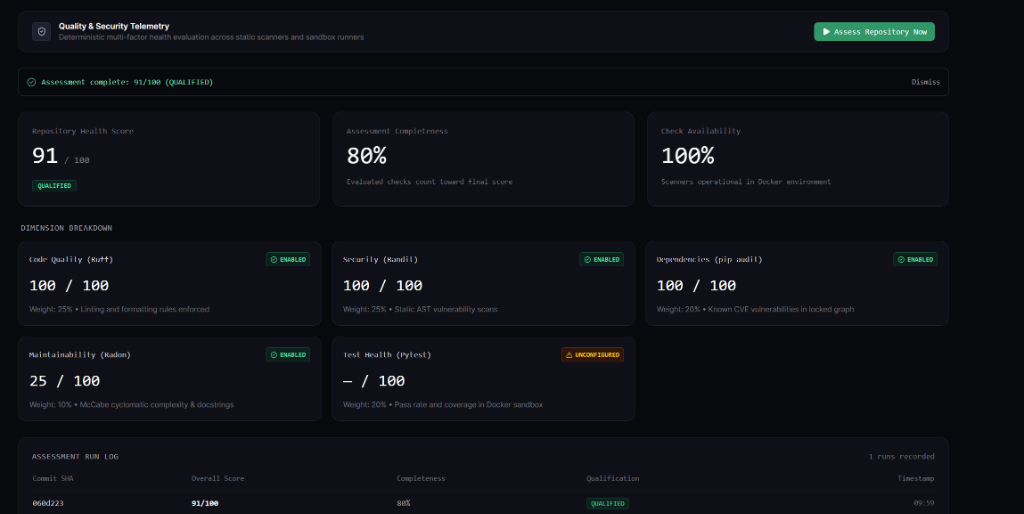
\includegraphics[width=0.88\textwidth]{images/screenshots/health_telemetry_qualified.png}
    \caption{MergeMind Health Telemetry View displaying a Qualified 91/100 Repository Assessment (Completeness: 80\%)}
    \label{fig:ui-telemetry-qualified}
\end{figure}

